\section{Цель работы}
Изучение инструментальных средств идентификации объектов управления.

\section{Задачи}
\subsection{Моделирование и имитация релейных систем управления}
Проведите анализ результатов, включающий следующие пункты:

\begin{enumerate}
	\item Анализ установившегося режима
	\item Частота колебаний в установившемся режиме
	\item Амплитуда колебаний в установившемся режиме
	\item Процедуру измерений п.2 и п. 3
	\item Анализ реализации релейного регулятора относительно теории
	\item Построение фазового портрета системы
\end{enumerate}

Замените регулятор на идеальное реле и повторите анализ системы

\subsection{Анализ устойчивости положений равновесия нелинейных систем}

\subsubsection{Задание 1}

Проанализируйте первым и вторым методом Ляпунова нелинейный осциллятор, заданный следующей системой дифференциальных уравнений
$$
\begin{cases}
	\frac{dV_1}{dt} = V_2, \\
	\frac{dV_2}{dt} = -2 \cdot V_1 -V_2^3
\end{cases}
$$

Проверьте себя, построив фазовый портрет системы и проанализировав его

\subsubsection{Задание 2}

Проанализируйте первым и вторым методом Ляпунова систему, заданную следующей структурной схемой:

\begin{figure}[H]
	\centering
	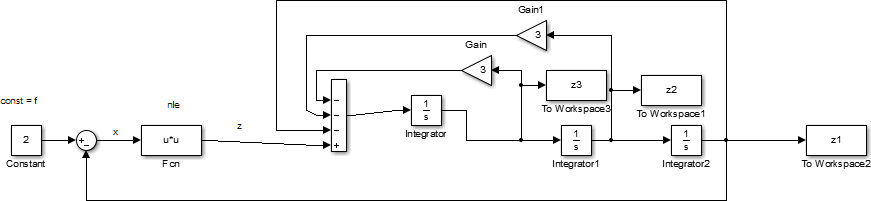
\includegraphics[width=0.9\linewidth]{body/images/non-linear-system.png}
\end{figure}

Для выполнения задания вам необходимо составить по схеме систему дифференциальных уравнений

Проверьте себя, построив фазовый портрет системы и проанализировав его

\section{Основные теоретические положения}

\subsection{Пример релейной системы стабилизации температуры}

Распространенными примерами систем управления, в которых некоторые сигналы принимают значения на конечных множествах, являются релейные системы. Релейные регуляторы — это простые и дешевые устройства, применяемые в несложных приложениях, например в термостатах отопительных систем и бытовых холодильников

Принципиальная схема релейной системы стабилизации температуры (термостата) изображена на изображении ниже.  Датчик температуры $\theta$ доставляет информацию о достижении пороговых значений $\theta_{min}$, $\theta_{max}$ и, тем самым, выделяет три ситуации (события):

\begin{enumerate}
	\item $\theta <\theta_{min}$ -  "Прохладно"
	\item $\theta_{min} < \theta <\theta_{max}$ - "Комфортно"
	\item $\theta >\theta_{max}$ - "Жарко"
\end{enumerate}

Управляющее воздействие  — напряжение, приложенное к нагревательному элементу, может принимать два значения 0 В (выключен) и 220 В (включен)

Система функционирует в условиях дефицита информации о состоянии объекта и минимального разнообразия управляющих воздействий. Алгоритм принятия решений выразим в форме правил:

\begin{enumerate}
	\item ЕСЛИ («Прохладно») ТО (Нагреватель включен)
	\item ЕСЛИ («Тепло») ТО (Нагреватель выключен)
	\item ЕСЛИ («Комфортно») И (Нагреватель включен) ТО (Нагреватель включен)
	\item ЕСЛИ («Комфортно») И (Нагреватель выключен) ТО (Нагреватель выключен)
\end{enumerate}

Ниже изображена статическая характеристика (СХ) релейного регулятора с гистерезисом для пороговых значений температуры $\theta_{min} = 21 ^{\circ}C$, $\theta_{max} = 23 ^{\circ}C$

\begin{figure}[H]
	\centering
	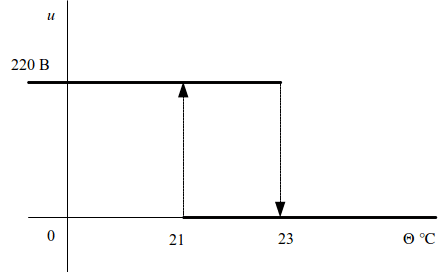
\includegraphics[width=0.7\linewidth]{body/images/relay.png}
\end{figure}

Обратим внимание на важное обстоятельство — если значения температуры принадлежат интервалу двузначности СХ, т. е. лежат между двумя пороговыми значениями, воздействие на объект определяется не только входом, но и состоянием объекта до того, как значение температуры вошло в этот интервал. Другими словами, выход регулятора определяется и предысторией, так как регулятор имеет память

Графическое задание даже двузначной СХ типа «реле с гистерезисом» дополняется комментариями о значениях выхода в зоне двузначности, например: 

$$
\begin{cases}
	C, x > b \\ 
	- C, x < -b \\
	C, |x|\leq b, y_0 = C \\
	-C, |x|\geq b, y_0 = -C
\end{cases}
$$

где: $b$ — половина зоны неоднозначности СХ; $y_0$ — состояние реле, равное значению $y$ до входа в зону неоднозначности. Таким образом, этот безынерционный нелинейный элемент (НЭ) обладает памятью — значение его выхода определяется не только значением входа в тот же момент, но также и предысторией (состоянием) НЭ по уровню сигнала

Неоднозначность кусочно-постоянных СХ создает сложности формального описания релейных и логических алгоритмов управления моделями типа «вход-выход». Необходимы иные формы представления

\subsection{Механизм вывода в четкой логике}

Механизм вывода в четкой логике (Crisp-Logic Inference System) образован последовательным соединением детектора событий, блока логики и декодера, исполняющих информационную, алгоритмическую и исполнительную функции

\begin{figure}[H]
	\centering
	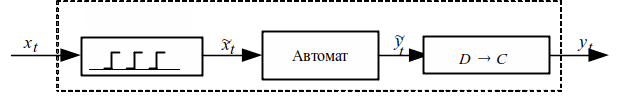
\includegraphics[width=0.7\linewidth]{body/images/logic-inference-system.png}
\end{figure}

Отображение непрерывного сигнала $x$ на множество символов $\widetilde{x}$ реализуется на пороговых элементах, разбивающих множества действительных значений на конечное число подмножеств. Пороги являются четкими, т. е. каждое значение входного сигнала может принадлежать строго одному подмножеству. Преобразователь $D \rightarrow C$ (декодер) сопоставляет выходным символам автомата  $\widetilde{y}_t$ действительные значения. Сигнал выхода $y_t$ представляет собой кусочно-постоянную функцию времени, уровень которой может изменяться с появлением нового символа на входе преобразователя

Моделью логических устройств, входы и выходы которых принимают значения из конечных множеств (символов), является автомат. Конечный автомат задается пятеркой   $<S, Y, X, \delta, \lambda>$ где $S, Y, X$ — множества состояний, выходов и входов автомата; $\delta$ — функция переходов; $\lambda$ — функция выходов. Функционирование автомата можно описать в терминах «вход-состояние-выход» 

$$
\begin{cases}
	\tilde{s}' = \delta(\tilde{s}, \tilde{x}); \tilde{s}_0, \\
	\tilde{y} = \lambda(\tilde{s}, \tilde{x})
\end{cases}
$$

Здесь $\tilde{s}'$ — последующее состояние, зависящее от предыдущего состояния $\tilde{s}$ и от входа $\tilde{x}$; $\tilde{s}_0$ — начальное состояние автомата

Механизмы вывода в четкой логике позволяют адекватно описать многозначные кусочно-постоянные преобразователи с разрывами первого рода и со сложной логикой переходов между ветвями СХ

Механизмы вывода в четкой логике описывают преобразования без временной памяти. Вместе с тем, внутренние состояния автомата позволяет учитывать «пространственную» память, выражаемую в многозначности преобразования — зависимости выхода от предыстории

Системы вывода в четкой логике — частный случай механизмов логического вывода на нечетких множествах (Fuzzy-Logic Inference Systems)

\subsection{Гибридные модели релейных систем управления}

Пример системы автоматической стабилизации температуры представляет систему, в которой сосуществуют как непрерывные переменные (температура), так и символьные последовательности, представляющие события (ситуации). Непрерывная часть системы описывается дифференциальными уравнениями, а моделью символьных преобразователей (логической части) являются конечные автоматы. Разнородные модели взаимодействуют посредством интерфейса, состоящего из двух частей — детектора событий $C \rightarrow D$ (измерительной части) и исполнительной части $D \rightarrow  C$

\begin{figure}[H]
	\centering
	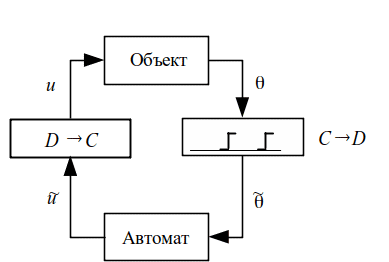
\includegraphics[width=0.7\linewidth]{body/images/hybrid-system.png}
\end{figure}

Такие системы называют гибридными. Гибридная модель типа Нероде―Кона (A. Nerode, W. Kohn) системы управления с обратной связью изображена на рисунке выше

\newpage

\section{Обработка результатов эксперимента}

\subsection{Моделирование и имитация релейных систем управления}

\textbf{Имитация релейной системы регулирования температуры}

Основным методом исследования систем управления по гибридным моделям является компьютерная имитация

Произведем компьютерную имитацию работы системы из примера:
$$
\begin{cases}
	T_1 \frac{dV}{dt} + v = u \\
	T_2 \frac{d\theta}{dt} + \theta = kv
\end{cases}
$$

где $T_1 = 20$  мин; $T_2 = 40$ мин;  $k = 40/220 ^{\circ}C/$В

Для имитации воспользуемся наработками из прошлых работ. И преобразуем систему дифференциальных уравнение в форму Коши:

\begin{figure}[H]
	\centering
	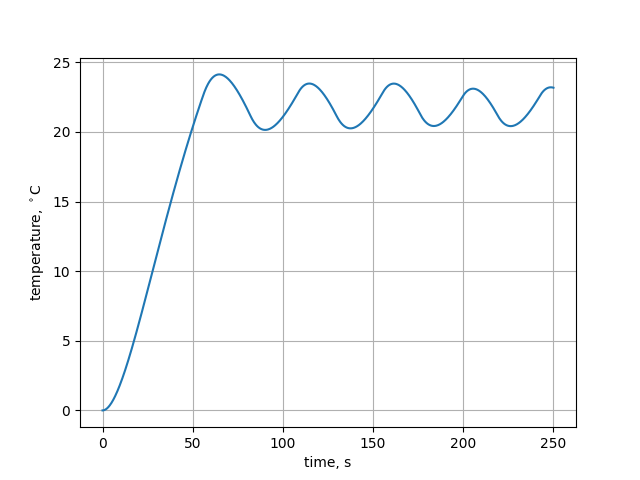
\includegraphics[width=1\linewidth]{body/images/default-system.png}
	\caption{Процесс при регуляторе с гистерезисом}
	\label{fig:1}
\end{figure}

Установившийся режим процесса представляет собой постоянное переключение между состоянием "вкл" и "выкл" нагревателя
при достижении граничных значений температуры - гармонический процесс

Для определения амплитуды колебаний, программно найдём максимальное и минимальное значения,
которых достигает температура. Используем алгоритм, похожий на градиентную эскалацию. Измерения
будет проводить после завершения переходного процесса. Амплитуда оказалась равной $1.39459906$. Также
программно был найден период колебаний, как величина, обратная постоянной времени. Постоянная времени определялась
таким же методом простейшей градиентной эскалации, и оказалась равна $43$ секундам. Тогда период колебаний будет равен
$ \approx 0.023256$ Гц

На рис. \ref{fig:2} представлен фазовый портрет системы с гистерезисом

\begin{figure}[H]
	\centering
	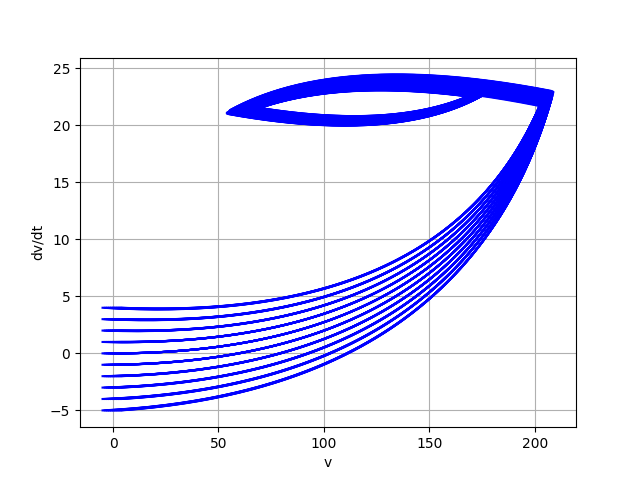
\includegraphics[width=1\linewidth]{body/images/default-system-phase-portrait.png}
	\caption{Фазовый портрет нагревательной системы с управляющим элементом с гистерезисом}
	\label{fig:2}
\end{figure}

Заменим регулятор на идеальное реле путем избавления от использования переменной состояния автомата

При использовании регулятора, реализующего реле в окрестности значений температуры в 23 $ ^{\circ}C $,
мы получаем колебательный процесс (Рис. \ref{fig:3}). Как можно заметить, этот колебательный процесс является
затухающим и связан с постоянно увеличивающейся частотой включения и выключения регулятора

\begin{figure}[H]
	\centering
	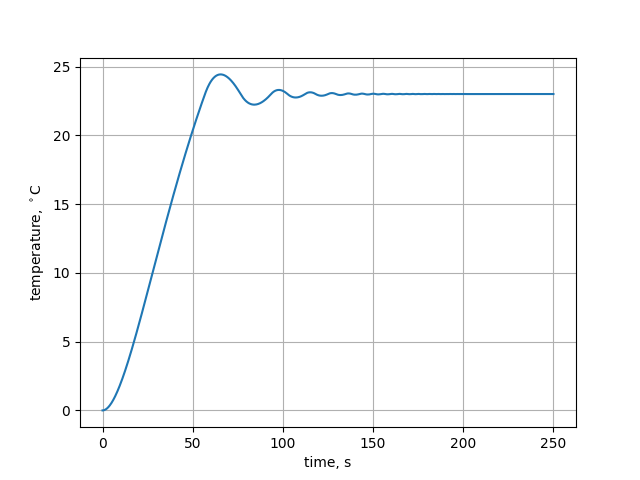
\includegraphics[width=1\linewidth]{body/images/relay-system.png}
	\caption{Процесс при регуляторе с реле}
	\label{fig:3}
\end{figure}

Как уже отмечалось выше, из-за того, что процесс является затухающим, нельзя точно говорить о частоте колебаний.
Данный вариант показывает большую предпочтительность по сравнению с гистерезисным регулятором. Однако, есть и минусы данного
подхода: на большом временном интервале количество переключений регулятора будет стремиться к бесконечности, что уже плохо.
Перенося это в реальность, можно сказать, что оборудование будет изнашиваться невероятно быстро, а значит такой подход
не может быть реализуем

На рис. \ref{fig:4} представлен фазовый портрет системы с реле

\begin{figure}[H]
	\centering
	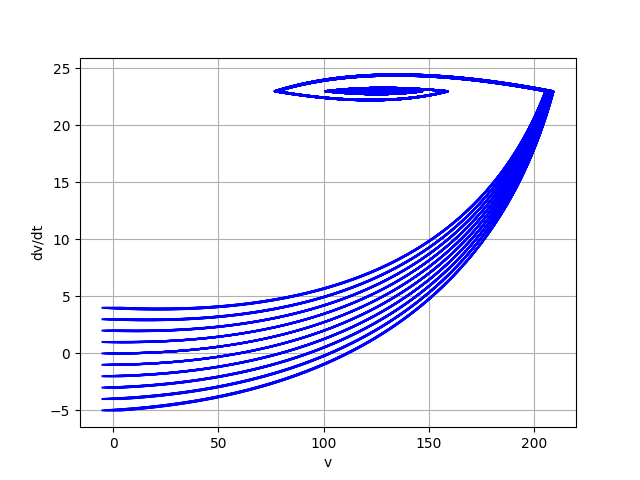
\includegraphics[width=0.8\linewidth]{body/images/relay-system-phase-portrait.png}
	\caption{Фазовый портрет нагревательной системы с управляющим элементом с реле}
	\label{fig:4}
\end{figure}

Если сравнивать вид фазовых портретов, то можно отметить то, что точкой стремления системы с элементом управления
с гистерезисом более всего является что-то похожее на особую точку "Центр". Точкой стремления системы с элементом управления
с реле явно видной особой точкой является особая точка "Устойчивый фокус". Перелом у каждой траектории
происходит на отметке 23, что говорит нам о сходстве с теорией

\subsection{Анализ устойчивости положений равновесия нелинейных систем}

\subsubsection{Задание 1}

Нелинейный осциллятор задан следующей системой дифференциальных уравнений:
$$
\begin{cases}
	\frac{dV_1}{dt} = V_2, \\
	\frac{dV_2}{dt} = -2 \cdot V_1 -V_2^3
\end{cases}
$$

Проанализируем устойчивость его положения равновесия первым методом Ляпунова
Для начала линеаризуем систему:
$$
\begin{cases}
	\frac{dV_1}{dt} = V_2, \\
	\frac{dV_2}{dt} = -2 \cdot V_1
\end{cases}
$$

У системы присутствует одна точка равновесия: $(0, 0)$.
Матрица Якоби будет иметь вид:

$$
A = 
\begin{pmatrix}
	0 & 1 \\
	-2 & 0
\end{pmatrix}
$$

Вычислим её собственные значения:

$$
det(sE - A) = s^2 + 2
$$

Найдя корни полинома, получим $s_{1,2} = \pm \sqrt2i$.
Корни мнимые, в этом критическом случае по линеаризованной модели нельзя судить
об устойчивости положения равновесия нелинейной системы

Проанализируем данную систму при помощи второго метода Ляпунова

Подберём функцию Ляпунова для двух переменных. Функция $V(V_1,V_2) = V_1 ^2 + \frac{1}{2}V_2 ^2$
удовлетворяет условиям теоремы Ляпунова об устойчивости

Найдём частные производные:

$\frac{dV(V_1,V_2)}{dV_1}=2 \cdot V_1$

$\frac{dV(V_1,V_2)}{dV_2}=V_2$

Найдём производную функции по времени:

$
\frac{dV(V_1,V_2)}{dt}=\frac{dV(V_1,V_2)}{dV_1} \cdot \frac{dV_1}{dt} + \frac{dV(V_1,V_2)}{dV_2} \cdot \frac{dV_2}{dt}
$

$
\frac{dV(V_1,V_2)}{dt}=2 \cdot V_1 \cdot V_2 + V_2 \cdot (-2 \cdot V_1 - V_2 ^3)
$

$
\frac{dV(V_1,V_2)}{dt}=-2 \cdot V_2 ^ 4 < 0
$

Следовательно, положение равновесия асимптотически устойчиво. Это проверяется также и с помощью фазового
портрета (Рис. \ref{fig:5}), по кооторому видно, что траектрии сходятся к точке $(0,0)$

\begin{figure}[H]
	\centering
	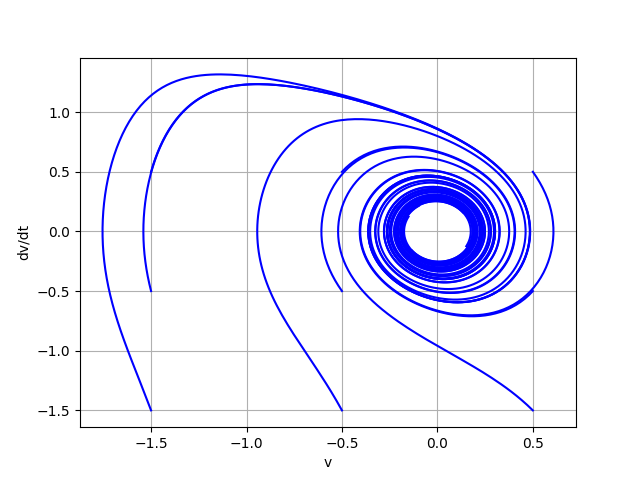
\includegraphics[width=0.7\linewidth]{body/images/non-linear-oscillator-system-phase-portrait.png}
	\caption{Фазовый портрет нелинейного осциллятора}
	\label{fig:5}
\end{figure}

\subsubsection{Задание 2}

Рассмотрим систему второго порядка, описанную блок-схемой (Рис. \ref{fig:6})

\begin{figure}[H]
	\centering
	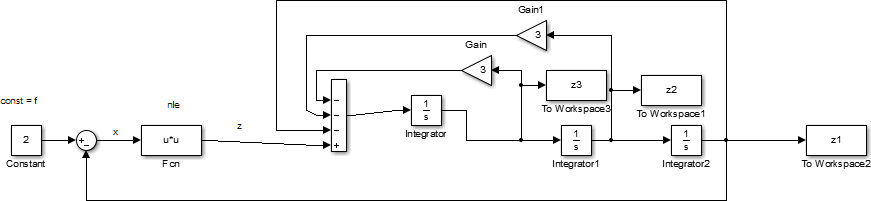
\includegraphics[width=0.8\linewidth]{body/images/non-linear-system.png}
	\caption{Блок-схема системы третьего порядка}
	\label{fig:6}
\end{figure}

Соответствующая система дифференциальных уравнений:

$$
\begin{cases}
	\frac{dz_1}{dt} = z_2, \\
	\frac{dz_2}{dt} = z_3, \\
	\frac{dz_3}{dt} = (2 - z_1)^2 - z_1 - 3 \cdot z_2 - 3 \cdot z_3
\end{cases}
$$

Проанализируем устойчивость его положения равновесия первым методом Ляпунова

Проверим положение равновесия системы. Корни уравнений: (1, 0, 0) и (4, 0, 0), рассмотрим их локально.

Для случая с $z_1 = 1$, система будет:
$$
\begin{cases}
	\frac{dz_1}{dt} = z_2, \\
	\frac{dz_2}{dt} = z_3, \\
	\frac{dz_3}{dt} = (2 - (z_1 - 1))^2 - (z_1 - 1) - 3 \cdot z_2 - 3 \cdot z_3
\end{cases}
$$

$$
\begin{cases}
	\frac{dz_1}{dt} = z_2, \\
	\frac{dz_2}{dt} = z_3, \\
	\frac{dz_3}{dt} = z_1^2 - 3 \cdot z_1 - 3 \cdot z_2 - 3 \cdot z_3
\end{cases}
$$

Для начала линеаризуем систему:
$$
\begin{cases}
	\frac{dz_1}{dt} = z_2, \\
	\frac{dz_2}{dt} = z_3, \\
	\frac{dz_3}{dt} = - 3 \cdot z_1 - 3 \cdot z_2 - 3 \cdot z_3
\end{cases}
$$


Характеристическая матрица будет иметь вид:

$$
A = 
\begin{pmatrix}
	0 & 1 & 0 \\
	0 & 0 & 1 \\
	-3 & -3 & -3
\end{pmatrix}
$$

Вычислим её собственные значения:

$$
det(sE - A) = -s^3-3 \cdot s^2-3 \cdot s-3
$$

Найдя корни полинома, получим $s_1 = -\sqrt[3]2-1$ $s_2 = \frac{-i \sqrt{3} \sqrt[3]{2} + \sqrt[3]{2} - 2}{2}$ $s_2 = \frac{i \sqrt{3} \sqrt[3]{2} + \sqrt[3]{2} - 2}{2}$ - два корня комплексно-сопряженные,
с отрицательной действительной частью и один отрицательный корень без мнимой части.
Получается, линеаризованная система асимптотически устойчива и положение равновесия нелинейной системы устойчиво "в малом" в точке (1, 0, 0)

Для случая с $z_1 = 4$, система будет:
$$
\begin{cases}
	\frac{dz_1}{dt} = z_2, \\
	\frac{dz_2}{dt} = z_3, \\
	\frac{dz_3}{dt} = (2 - (z_1 - 4))^2 - (z_1 - 4) - 3 \cdot z_2 - 3 \cdot z_3
\end{cases}
$$

$$
\begin{cases}
	\frac{dz_1}{dt} = z_2, \\
	\frac{dz_2}{dt} = z_3, \\
	\frac{dz_3}{dt} = z_1^2 + z_1 - 3 \cdot z_2 - 3 \cdot z_3
\end{cases}
$$

Линеаризуем систему:
$$
\begin{cases}
	\frac{dz_1}{dt} = z_2, \\
	\frac{dz_2}{dt} = z_3, \\
	\frac{dz_3}{dt} = z_1 - 3 \cdot z_2 - 3 \cdot z_3
\end{cases}
$$

Характеристическая матрица будет иметь вид:

$$
A = 
\begin{pmatrix}
	0 & 1 & 0 \\
	0 & 0 & 1 \\
	1 & -3 & -3
\end{pmatrix}
$$

Вычислим её собственные значения:

$$
det(sE - A) = -s^3-3 \cdot s^2-3 \cdot s+1
$$

Найдя корни полинома, получим $s_1 = \sqrt[3]2-1$ $s_2 = \frac{-i \sqrt{3} \sqrt[3]{2} - \sqrt[3]{2} - 2}{2}$ $s_2 = \frac{i \sqrt{3} \sqrt[3]{2} - \sqrt[3]{2} - 2}{2}$ - два корня комплексно-сопряженные,
с отрицательной действительной частью и один положительный корень без мнимой части.
Следовательно, положение равновесия нелинейной системы неустойчиво в точке (4, 0, 0)

Проанализируем данную систму при помощи второго метода Ляпунова

Подберём функцию Ляпунова для трёх переменных:

$
V(V_1,V_2,V_3)=\frac{1}{2}(Z_1^2+Z_2^2+Z_3^2)
$

Найдём частные производные функции:

$
\frac{dV(Z_1,Z_2,Z_3)}{dZ_1}=Z_1
$

$
\frac{dV(Z_1,Z_2,Z_3)}{dZ_2}=Z_2
$

$
\frac{dV(Z_1,Z_2,Z_3)}{dZ_3}=Z_2
$

Найдём производную функции по времени:

$
\frac{dV(Z_1,Z_2,Z_3)}{dt}=
\frac{dV(Z_1,Z_2,Z_3)}{dZ_1} \cdot \frac{dZ_1}{dt} + 
\frac{dV(Z_1,Z_2,Z_3)}{dZ_2} \cdot \frac{dZ_2}{dt} + 
\frac{dV(Z_1,Z_2,Z_3)}{dZ_3} \cdot \frac{dZ_3}{dt} + 
$

$
\frac{dV(Z_1,Z_2,Z_3)}{dt}=Z_1 \cdot Z_2 + Z_2 \cdot Z_3 - Z_3 \cdot (4-3 \cdot Z_1 - 3 \cdot Z_2 - 3 \cdot Z_3 + Z_1^2)
$

$
\frac{dV(Z_1,Z_2,Z_3)}{dt}=4 \cdot Z_3 + Z_1Z_2 - 2 \cdot Z_2Z_3 - 3 \cdot Z_1Z_3 - 3 \cdot Z_3^2 + Z_3Z_1^2
$

Преобразовать уравнение так, чтобы можно было однозначно сказать о знаке выражения, нельзя. Следовательно, и об устойчивости - тоже

Проверим результат применения первого метода Ляпунова, построив фазовый портрет системы (рис. \ref{fig:7}).
Поведение траекторий напоминает такие особые точки как устойчивый фокус в точке $(1, 0, 0)$ и седло в точке $(4, 0, 0)$.
Заметно большое влияние седла, так как многие траектории уходят в бесконечность

\begin{figure}[H]
	\centering
	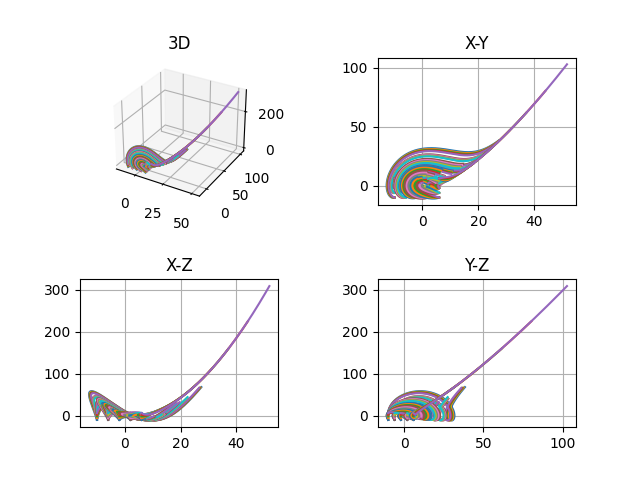
\includegraphics[width=1.1\linewidth]{body/images/third-order-system.png}
	\caption{Фазовый портрет системы третьего порядка}
	\label{fig:7}
\end{figure}

\newpage

\section{Выводы}

В ходе работы было смоделировано и проанализировано поведение релейной системы управления с внутренней памятью и
системы с идеальным реле, а также были применены методы Ляпунова: первый и второй